\documentclass[a4paper, 12pt]{article}
\usepackage[slovene]{babel}
\usepackage[utf8]{inputenc}
\usepackage{minted}
\usepackage{nameref}
\usepackage[backend=bibtex]{biblatex}
\usepackage{graphicx}

\graphicspath{{images/}}

\title{
    Programiranje v Pythonu\\\large
    Izdelava programa za steganografijo slik}
\author{Matej Marinko}
\date{februar 2017}


\addbibresource{latex/viri.bib}

\begin{document}
    \maketitle
    \thispagestyle{empty}
    \newpage

    \begin{abstract}
        % Namen naloge je ugotoviti, \ldots
    \end{abstract}
    \newpage

    \tableofcontents
    \newpage

    \section{Uvod} 

    \newpage 

    \section{Steganografija}
        Steganografija je znanost, ki omogoča skrivanje podatkov v navidezno nepomembnem prenosnem mediju. Beseda izhaja iz grščine, in pomeni ``zakrito pisanje''. Predstavlja skupek metod za skrivanje informacij v neke druge informacije. Za razliko od kriptografije oz. šifriranja, ki želi podatke narediti neberljive, steganografija poskuša prikriti, da ti podatki sploh obstajajo \cite{monitor}.

Šibkost kriptografije je, da je sporočilo sumljivo že na prvi pogled. Šibkost steganografije pa je, da ko nekdo enkrat odkrije, kje je sporočilo skrito, ga lahko enostavno prebere. V praksi se zato pogosto uporabljata obe metodi skupaj, saj druga drugi odpravita slabosti.

\subsection{Tehnike}
    Primeri steganografije so znani že od Antike, različne tehnike pa so se ohranile vse do danes. Z razvojem računalništva se je steganografija razvila tudi na digitalnem področju.\\

    \textbf{Primeri fizičnih tehnik:}
    \begin{itemize}
        \item V Stari Grčiji so sporočila skrivali v voščene tablice. Na les so napisali sporočilo, ki so ga nato prekrili z voskom. Na vosek pa so napisali nedolžno in nepomembno sporočilo.
        \item Drugi postopek, ki so ga uporabljali v Antični Grčiji je bil približno takšen: Sužnju so pobrili glavo in mu vtetovirali sporočilo. Ko so lasje zrasli sporočilo ni bilo več vidno. Očitna pomankljivost te metode je, da moramo počakati, da osebi lasje zrastejo nazaj.
        \item Sporočilo, ki je napisano z nevidnim črnilom, na nepopisanem delu pisma.
        \item Sporočilo je v Morsejevi abecedi, napisani na prejo, ki so jo potem vtkali kurirju  v blago.
        \item Del črk v besedilu je napisan z drugačno pisavo kot druge črke (npr. ležeče). Te črke so tvorile skrivno sporočilo. \cite{wikipedia}
        \item Nemci so med drugo svetovno vojno uporabljali mikropike (microdots). Podatke so skrivali v znakih, ki jih je bilo mogoče prebrati samo pod veliko povečavo. \cite{monitor}
        \item Cardanovo rešeto - mreža z odprtinami, s katero prekrijemo besedilo, da se prikaže skrito sporočilo.
        \item Ameriški pilot Jeremiah Denton, ki ga je ujela vietnamska vojska, je bil med televizijsko konferenco prisiljen pričati, da z njim v ujetništvu ravnajo dobro. Hkrati pa je z mežikanjem v morsejevi abecedi črkoval besedo T-O-R-T-U-R-E (mučenje).\cite{delo}
    \end{itemize}

    \textbf{Primeri digitalnih tehnik:}
    \begin{itemize}
        \item Skrivanje podatkov v najnižje bite slikovnih datotek, z neopaznimi spremembami barv.
        \item Skrivanje podatkov v zvočni zapis, s spremembami, neslišnimi za človeško uho.
        \item Tehnika ``pletja in presejanja'' (chaffing and winnowing), kjer gre za to da paketkom, ki gredo čez nezavarovano povezavo dodamo lažne paketke, v katere lahko skrijemo sporočilo.
        \item Dodajanje podatkov v neuporabljene sektorje na disku, ali na konce sektorjev.
        \item Skrivanje z uporabo unicode znakov, ki izgledajo enako kot ASCII znaki.
        \item Nekateri moderni tiskalniki z težko vidnimi svetlo rumenimi pikami na vsakem listu označijo serijsko številko tiskalnika in čas tiska.
        \cite{wikipedia}
    \end{itemize}

\subsection{Steganografija digitalnih fotografij}
    \label{steganografijaslik}
    Večja kot je datoteka, v katero nameravamo skriti naše sporočilo, v primerjavi z tem sporočilom, lažje jo je skriti. Zato so slike primerne za steganografijo, saj vsebujejo velike količine podatkov. Tako lahko skrijemo podatke npr. na Internetu. Slika je vsem na očeh, venar se nihče ne zaveda, da so v njej skrite še dodatne informacije. Ni znano, kako pogosta je ta praksa, vendar vemo da obstaja.
    
    V RGBA zapisu uporabimo 32 bitov za vsak piksel, to pomeni 8 bitov za vsako komponento. Samo rdeča barva ima $2^8$ različnih intenzivnosti. (Glej poglavje: \nameref{zapisslik}) Razliko med $10111111_{(2)}$ in $10111110_{(2)}$ v inteziteti barve človeško oko zelo težko prepozna. Zato lahko najnižje bite (least significant bits) spremenimo in v njih skrijemo svoje podatke. Če v vsakem pikslu v vseh štirih komponentah spremenimo 2 najmanj pomembna bita, lahko v en piksel skrijemo 1 bajt (8 bitov) podatkov. V celotni sliki lahko, če je dovolj velika, skrijemo tudi več MB podatkov.

    Pri tem je pomembno, da slika, v katero želimo skriti podatke ni enobarvna, oziroma sestavljena iz večjih enobarvnih ploskev. Če je slika takšna, obstaja večja možnost, da kdo opazi različne odtenke sosednjih pikslov na sliki. Zato so slike, ki se uporabljajo za steganografijo pogosto slike narave, živali, ipd.

\subsection{Steganaliza}
    Steganaliza je veda, ki se ukvarja z zaznavanjem sporočil, skritih s pomčjo steganografije. Pogosto se povezuje s kriptoanalizo. Namen je torej najti sumljiva sporočila, ter ugotoviti ali se v njih skriva skrito sporočilo in, če je možno, prebrati to sporočilo.

    Problema se ponavadi lotimo z statistično analizo. Analiziramo recimo slike, ki so bile posnete z enakim fotoaparatom, ali zvočne posnetke in ugotavljamo skupne značilnosti. Zaradi pogoste izgubne kompresije je predvidljivo, kakšni naj bi bili podatki. V JPEG sliki, naprimer, lahko precej dobro sklepamo, katere barve je piksel, če poznamo vse sosednje piksle. Ker so takšne razporeditve predvidljive, bodo slike, v katerih je skrito stenografsko sporočilo hitreje opazne.

    Najlažje pa je odkriti skrito sporočilo, če imamo na voljo originalno sliko, v kateri ni skritih podatkov, saj bomo hitro opazili razliko in bomo posledično lažje izluščili podatke.

    Še naprednejše metode predpostavijo, da so podatki, ki so skriti poleg tega še kriptirani. Posledica sodobne enkripcije je, da so podatki videti naključni. Večina metod skriva podatke v najmanj pomembne bite (least-significant bits). Če bo razporeditev 1 in 0 v najmanj pomembnih bitih skoraj popolnoma naključna, je velika verjetnost, da je v datoteki skrito kriptirano sporočilo.


          
    \section{Zapis slik v računalniku}
        \label{zapisslik}
Slika je v računalniku zapisana tako, da je razdeljena na drobne kvadratke, imenovane piksli. Vsak piksel ima podatke kako močno in v katerih barvah žari. Za zapis se uporablja več različnih formatov, med katerimi so najbolj znani JPEG, PNG, BMP, GIF\ldots Med seboj se razlikujejo v različnih lastnostih, kot so način zgoščevanja, število možnih barv posameznega piksla\ldots

Osnovna zgradba vsakega formata sestoji iz:
\begin{description}
    \item [glave,] ki vsebuje glavne podatke, kot so velikost, barvna globina in kompresijska tehnika. 
    \item [slikovnih podatkov] oziroma niza pikslov. Podatki so lahko kompresirani ali nekompresirani.
    \item [polj za metapodatke] (metadata), kot so datum posnetka, avtor slike\ldots
\end{description} 

\subsection{Format PNG}
    PNG (Portable Network Graphics) je razmeroma nov slikovni format, ki je popularen predvsem na spletu.

    Format PNG uporablja brezizgubno kompresijo, kar nujno potrebujemo pri steganografiji, saj se zanašamo na to da bomo podatke lahko skrili tako, da jih človeško oko ne bo zaznalo. Izgubna kompresija pa izpušča podatke, ki jih človeško oko ne more zaznati, ter tako onemogoča pridobivanje skritega sporočila nazaj iz slike.

    Ena izmed prednosti formata PNG pred drugimi slikovnimi formati je podpora več različnih barvnih tabel. Poleg standardnega RGB (Red Blue Green) zapisa podpira tudi RGBA (Red Green Blue Alpha) zapis, katerega bistvena razlika je dodaten alpha kanal. Le-ta se navadno uporablja za prosojnost slik. Če je vrednost kanala 0\% je piksel popolnoma prosojen, če pa je vrednost 100\% pa je piksel enak običajnim pikslom.

    V primeru steganografije dodaten kanal veliko pripomore, saj lahko v sliko skrijemo kar $\frac{1}{4}$ več informacij, kot v zapisu RGB (Glej poglavje: \nameref{steganografijaslik}).


    \section{AES kriptiranje}
        AES (Advanced Encryption Standard) je eden najbolj uporabljenih standardov za simetrično enkripcijo. Simetrična enkripcija pomeni, da imata pošiljatelj in prejemnik isti ključ, s katerim kriptirata oziroma dekriptirata sporočilo. 

Algoritem sta razvila belgijska kriptografa Joan Daemen in Vincent Rijmen, ter ga poimenovala Rijndael. Pozneje je standard z manjšimi spremembami prevzela ameriška vlada kot naslednji standard po uporabi DES (Data Encryption Standard), saj so ključi DES postali prekratki in jih je bilo mogoče razbiti z močnejšimi računalniki.

AES je ``substitution-permutation network'', kar pomeni, da glavnino operacij, ki jih opravlja predstavljajo različne zamenjave in permutacije bitov.   

Poleg višje varnosti je glavna prednost standarda AES hitrost. Operacije, ki jih opravlja so nezahtevne, v nasprotju z asimetričnimi kriptiranji. AES pa je v nasprotju z njimi možno zapisati v vezje v procesorju, tako da lahko današnji običajni namizni računalniki kriptirajo AES tudi z več TB/s.

\subsection{Algoritem}
    Algoritem poenostavljeno sestoji iz štirih korakov, ki se naprej delijo na manjše korake.
    \begin{enumerate}
        \item \texttt{KeyExpansions} - razširitve ključa. Ključ, ki je vnaprej določene dolžine se razširi na več ključev, saj AES za vsak krog zahteva svoj ključ.
        \item \texttt{InitialRound} - dodajanje ključa. Nastavjo se začetna stanja s pomočjo posameznih delov ključa.
        \item \texttt{Rounds} - del, ki se večkrat ponovi, vsakokrat z novim ključem, ki smo ga razširili iz originalnega ključa. Če je ključ 128-biten se ponovi 10-krat, 12-krat pri 192-bitnih ključih in 14-krat pri 256-bitnih ključih.
            \begin{enumerate}
                \item \texttt{SubBytes} - preprosta substitucija znakov z uporabo tabele. Pri tem je pomembno, da ime tabela določene lastnosti, ki naredijo to preslikavo nelinearno, kar zelo oteži razbijanje šifre.
                \item \texttt{ShiftRows} - operacija na vrsticah trenutnega stanja. Vsak bit v neki vrstici se ciklično zamakne za neko število. Biti iz konca se premaknejo na začetek.
                \item \texttt{MixColumns} - korak, kjer se stolpci zamenjajo z drugimi stolpci. Vsa stanja v novem stolpcu so neposredno odvisna od vsakega posameznega stanja v prvotnem stolpcu. Če spremenimo en znak, se popolnoma spremeni celoten novi stolpec.
                \item \texttt{AddRoundKey} - korak skoraj enak postopku v InitialRound. Stanju se doda nov ključ, ki ustreza trenutnemu krogu, z operacijo \texttt{XOR} (ekskluzivni ali).
            \end{enumerate}
        \item \texttt{Final Round} - še zadnja ponovitev, ki je skoraj enaka vsem ostalim krogom, edina razlika je, da ne vsebuje koraka \texttt{MixColums}.\cite{wikipedia-aes}
    \end{enumerate}

    \section{Python}
        Python je sodoben programski jezik, ki je primeren za razvoj najrazličnejših programov, od preprostih skript do numerično zahtevnih simulacij in sodobnih spletnih aplikacij. Zaradi svoje enostavnosti je postal eden najpriljubljenejših programskih jezikov vseh časov, ter je primeren za učenje programiranja. Python je tolmačen jezik, to pomeni, da se sproti med izvajanjem pretvarja v strojno kodo.\cite{rin} Zato je razmeroma počasnejši od prevajanih jezikov, kot so C++, Java in C\#. V praksi se z uporabo različnih knjižnjic, kot je numpy, njegova hitrost izvajanja lahko približa hitrosti teh jezikov.

Prednost (in hkrati tudi slabost Pythona) je uporaba dinamičnih tipov, kar pomeni, da imamo lahko v isti spremenljivki ob različnih časih različne podatkovne tipe. Sintaksa Pythona omogoča, da razvijalci prišejo kodo hitreje kot v drugih programskih jezikih, saj potrebujejo manj vrstic kode kot v konkurenčnih jezikih.

\subsection{Verzije Pythona}
    Python trenutno obstaja v dveh glavnih verzijah. To sta 2.x in 3.x (v nadaljevanju tudi Python2 in Python3). Verzija Python3 je novejša, bolj optimizirana, v njej so tudi popravili nekaj pomembnih ``napak'', ki so bile v Python2. Pomembnejše izboljšave v Python3 so:
    \begin{itemize}
        \item Podpora Unicode znakov. Unicode znaki so lahko vključeni v nizih in tudi v imenih spremenljivk.
        \item Pravilnejša implementacija nekaterih delov osrednjih jezika - \texttt{print} in \texttt{exec} nista več stavka (statements), temveč funkciji. Deljenje dveh celih števil vrne racionalno število.
        \item Optimizacije delovnega spomina - različne funkcije (\texttt{range()}, \texttt{map()}, \texttt{filter()} \ldots) vrnejo iteracijske objekte, namesto da bi ustvarile celotne sezname.
        \item Besedi \texttt{True} in \texttt{False} sta rezervirani in jih programer ne more več po nesreči spreminjati.
    \end{itemize}

    Python3 ima veliko prednosti in skoraj nobene slabosti v primerjavi z Pythonom2. Ena od slabosti je, da je za majhna števila malo počasnejši kot Python2, saj ne uporablja tipov \texttt{int} ampak tipe \texttt{long}, ki zahtevajo več spomina in novejše procesorje. Poleg tega je za Python3 na razpolago manjše število različnih knjižnjic kot za Python3, vendar ta razlika skoraj ni več opazna, saj je tudi od nastanka Pythona3 minilo že kar nekaj let in ga uporablja vedno več razvijalcev.

\subsection{Knjižnjice}
    Python-ova standardna knjižnjica je razmeroma velika, že vsebuje orodja za veliko različnih nalog. Vsebuje že knjižnjice za izdelavo preprostih internetnih aplikacij, grafičnih vmesnikov in tudi knjižnjici za poganjanje testov.

    Veliko programov pa ni vključenih v Pythonovo standardno knjižnjico, vendar jih je zato še več v PyPI (Python Package Index), kjer je trenutno (februarja 2017) 99610 različnih paketov. Z različnimi moduli si poenostavimo pisanje programa, saj nam ni treba ponovno implementirati celotnih funkcij, ki bi jih potrevali. Nekateri moduli pa nam omogočijo stvari, ki jih v ``čistem Pythonu'' sploh ne moremo napisati, oziroma so napisani deloma v drugem programskem jeziku zato, da se naš program izvaja hitreje.

    Pomembnejše knjižnjice za izdelavo programa steganografije slik:
    \begin{description}
        \item [Pillow:] Knjžnjica za delo z različnimi formati slik. Povzeta po knjižnjici \texttt{PIL} (Python Imaging Library), ki je napisana za Python verzije 2.x, medtem ko je Pillow namenjena za verzije 3.x.
        \item [PyCrypto] Zbirka varnih hash funkcij in različnih kriptirnih algoritmov (RSA, AES, DES\ldots).
        \item [Tkinter] Pythonova standardna knjižnjica za izdelavo grafičnega uporabniškega vmesnika (GUI).
    \end{description}


    \section{Izdelava programa}
        \subsection{Priprava okolja}
    Sam sem pri programiranju uporabljal operacijski sistem Ubuntu, popularno distribucijo Linuxa, ker je po mojem mnenju programiranje na Linuxu veliko lažje in bolj praktično kot na Windowsih. Tudi programski jezik Python je že prednaložen na večini Linux distribucijah, tako verzija 2.x kot 3.x. Program je napisan v Pythonu verzije 3.5.

    Najprej naložimo knjižnjici, ki jih potrebujemo:

    \inputminted[firstline=1, lastline=2, frame=lines]{bash}{latex/bashscripts.sh}

    Za pisanje kode sem uporabljal odprtokodni program Atom (\texttt{https://atom.io/}), za upravljanje verzij pa program Git, v povezavi z shrambo v oblaku Github (\texttt{www.github.com}). 


\subsection{Pridobivanje podatkov}

    Program od uporabnika pridobi podatke, v katero sliko želi skriti podatke in datoteko s podatki, ki jo želi skriti. Po mojem mnenju je veliko bolje, če lahko v sliko skrijemo katere koli podatke, ne samo besedila. Ko program pridobi ime datoteke, jo odpre kot \texttt{bytes} objekt z imenom \texttt{secret}. 

    \inputminted[firstline=1, lastline=2, frame=lines]{python}{latex/code_parts.py}

    V tem primeru je bolj ``varno'' uporabiti stavek \texttt{with}, saj nam Python samodejno zapre datoteko, ko program konča delo v tistem scopu. Tako ne pride do nenamerne prekomerne porabe spomina, saj imamo datoteko odprto samo toliko časa kot jo res potrebujemo.


\subsection{Pridobivanje gesla}

    Program uporabnika vpraša za geslo, s katerim želi zakriptirati datoteko. Ker v običajnem načinu terminala lahko vidimo, kaj uporabnik vpisuje v terminal, ampak ne želimo, da se vidi tudi geslo, moramo v brezgrafičnem načinu uporabiti posebno Pythonovo knjižnjico \texttt{getpass}.  

    \inputminted[firstline=4, lastline=5, frame=lines]{python}{latex/code_parts.py}

    Ko bo uporabnik vpisoval geslo, se ga ne bo videlo, a bo še vedno spravljeno v spremenljivki geslo. Ker so Pythonove spremenljivke globalno dostopne, je bolje, če gesla ne shranimo v ločeno spremenljivko, saj načeloma lahko nek drug del našega programa dostopa do uporabnikovega gesla. Bolje je če geslo takoj podamo funkciji, ki bo iz gesla naredila \texttt{sha256 hash}.

    \inputminted[firstline=7, lastline=7, frame=lines]{python}{latex/code_parts.py}

    V grafičnem vmesniku \texttt{tkinter} pa objektu \texttt{Entry} dodamo lastnost, da namesto gesla, ki ga vpisuje uporabnik prikaže samo nek znak, v tem primeru \texttt{*}.

    \inputminted[firstline=9, lastline=10, frame=lines]{python}{latex/code_parts.py}

    Ko programu s pritiskom na gumb \texttt{Hide} ali \texttt{Find} povemo, naj med drugim pridobi geslo, ga moramo potem izbrisati iz polja, da ne bi prišlo do kakšne zlorabe gesla.

    \inputminted[firstline=12, lastline=15, frame=lines]{python}{latex/code_parts.py}

    Pythonova funkcija \texttt{del()} izbriše določeno spremenljivko. Za stvari kot so gesla v nizih, je ponavadi bolje, če jih izbrišemo takoj ko jih ne potrebujemo več, namesto da čakamo, da to namesto nas naredi Python.


\subsection{Kriptiranje podatkov}

    Glavni del AES kriptiranja bo za nas opravila knjižnjica \texttt{PyCrypto}, saj je njihova implementacija kriptiranja zagotovo bolj pravilna od takšne, ki bi jo napisal jaz. Sama koda je popolnoma preprosta, vse se zgodi v funkciji \texttt{encrypt(message, key)}, pri čemer je \texttt{message} sporočilo, ki ga želomo zakriptirati, \texttt{key} pa je \texttt{sha256 hash} gesla.

    \inputminted[firstline=17, lastline=19, frame=lines]{python}{latex/code_parts.py}

    Paziti moramo le na to, da je dolžina celotnega sporočila, ki ga želimo zakriptirati z AES algoritmom deljiva z 16. Tudi ustvarjanje hasha je preprosto, saj skoraj vse za nas naredi knjižnjica \texttt{PyCrypto}.

    \inputminted[firstline=21, lastline=23, frame=lines]{python}{latex/code_parts.py}


\subsection{Skrivanje podatkov v sliko}
    Knjižnjica \texttt{PIL} (Pillow) nam omogoča, da s sliko delamo podobno, kot z dvodimenzionalnim seznamom. Najprej ustvarimo novo sliko, in potem za vsako vrstico in vsak stolpec prekopiramo piksel iz originalne slike \texttt{image\_data}. Dokler še nismo skrili celotnega sporočila (\texttt{if index < len(secret):}), vsakemu kanalu na sliki (\texttt{RGBA}) spremenimo zadnja dva bita v vrednost, ki jo potrebujemo.

    \inputminted[firstline=25, lastline=49, frame=lines]{python}{latex/code_parts.py}

    Zato, ker je pikslov v posamezni sliki veliko, uporabimo bitne operacije, ker so malo hitrejše, kot npr. operacije na celih številih. Cela števila si lahko predstavljamo v binarnem zapisu. Če želimo dobiti določene bite nekega števila (v tem primeru vse bite razen zadnjih dveh) uporabimo bitno operacijo and (\texttt{\&}) z enicami na tistih mestih, kjer želimo dobiti bite tistega števila in ničlo na tistih mestih, kjer želimo $0$ v vsakem primeru. Ker želimo dobiti vse bite razen zadnjih dveh, to pomeni, da želimo izvesti operacijo z številom $11111100_{(2)}$ oziroma negiranim številom $0$\ldots$011_{(2)} = 3$. Znak za negacijo v Pythonu pa je \texttt{\~}.

    \inputminted[firstline=51, lastline=51, frame=lines]{python}{latex/code_parts.py}

    Sedaj želimo na zadnji dve mesti, ki sta zagotovo $0$ skriti en bajt naših podatkov, kar pomeni, da bomo v vsako ``barvo'' skrili po dva bita. Če si predstavljamo, da naš bajt izgleda takole: $11001001_{(2)}$ in mi želimo dobiti po dva bita, to izgleda približno tako:

    $$11001001_{(2)} \wedge 00000011_{(2)} = 00000001_{(2)}$$
    $$11001001_{(2)} \wedge 00001100_{(2)} = 00001000_{(2)}$$
    $$11001001_{(2)} \wedge 00110000_{(2)} = 00000000_{(2)}$$
    $$11001001_{(2)} \wedge 11000000_{(2)} = 11000000_{(2)}$$

    Ker želimo te znake dodati na konec barv, moramo dobljena števila spremeniti še z operacijo \texttt{right shift}, v Pythonu \texttt{>>}. Ta operacija vse bite v številu premakne za določeno število v desno.

    $$11011100 \gg 2 = 00110111$$

    Ko naredimo to, samo še z operacijo or (\texttt{|}) dodamo bite barvnim kanalom in vse skupaj shranimo v piksel na novi sliki.

    \inputminted[firstline=53, lastline=53, frame=lines]{python}{latex/code_parts.py}


\subsection{Iskanje podatkov}
    Iskanje podatkov v sliki je precej podobno skrivanju podatkov. Prav tako najprej od uporabnika potrebujemo podatke, v kateri sliki želi iskati podatke, kam bo shranil najdene podatke in geslo. Ena od razlik je, da ko iščemo podatke v sliki, najprej ne vemo, koliko jih je, oziroma do katerega piksla so naši podatki. Zato so v slikah, v katerih so bili skriti podatki s tem programom v prvih 4 pikslih podatki o dolžini, datoteke, ki jo želimo skriti. To pomeni, da je najdaljši možen zapis, ki ga lahko skrijemo v sliko:

    $$(2^8)^4 = 256^4 = 4294967296 > 4 \cdot 10^9$$

    Pri velikosti slik, ki so danes nekaj čez 10 mio pikslov je torej dovolj, da si podatke o dolžini zapomnimo v samo 4 pikslih. 

    \inputminted[firstline=55, lastline=87, frame=lines]{python}{latex/code_parts.py}

    Potem, ko imamo podatke o dolžini skritega sporočila, samo dodajamo najdene podatke na seznam \texttt{secret}. Ko pridobimo vse podatke, pa moramo seznam še dekriptirati in dobimo sporočilo. Ker sporočilo ni nujno samo tekstovno, ga namesto, da bi ga izpisali na zaslonu, shranimo v datoteko, ki jo je poimenoval uporabnik. Zato lahko na ta način v eno sliko lahko skrijemo ne le preprostega besedila, ampak tudi druge dokumente ali celo druge slikovne datoteke.


\subsection{Primer uporabe programa}
    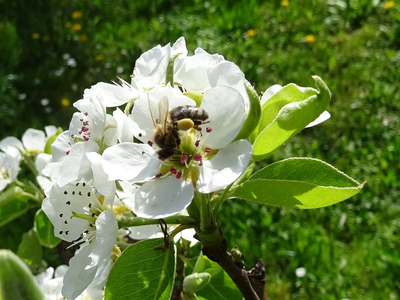
\includegraphics[width=0.5\textwidth]{image.png}
    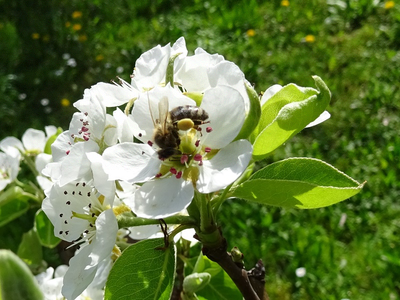
\includegraphics[width=0.5\textwidth]{image_with_hidden_data.png}

    Leva fotografija je samo fotografija čebele na cvetu, velika 400x300 slikovnih točk. Desna slika ji je na prvi pogled enaka, vendar je v njej skrito $10 000$ besed vzorčnega teksta (\textit{Lorem ipsum dolor sit amet\ldots}), zakriptiranih z geslom ``\texttt{geslo}''. Velikost datoteke, ki smo jo skrili je bila 68,1 kB. Prva slika je velika 254,5kB, druga pa 273,3 kB. Sliki se razlikujeta v velikosti, saj zaradi skritih podatkov v najnižjih bitih stiskanje podatkov ni bilo več tako zelo učinkovito. Razlika v velikosti v tem primeru ni bistvena, saj je prva slika že dovolj ``nepravilna'', da že prej ni bilo mogoče slike popolnoma stisniti. Če bi podatke skrivali v sliko, ki bi bila enobarvna, potem bi se velikost spremenila še bolj, poleg tega pa bi bilo s prostim očesom možno opaziti, da je v sliki nekaj skrito (slika ne bi bila več enbarvna, temveč bi bili sosednji piksli med seboj rahlo različnih barv).


    Program lahko uporabljamo na dva različna načina: v grafičnem načinu, ter v načinu ukazne vrstice.

    \subsubsection{Z ukazno vrstico}

        Recimo da imamo datoteko \texttt{slika.png}, v katero želimo skriti naše podatke, ki jih imamo spravljene v datoteki \texttt{skrivnost.txt}. Ime nove slike, v kateri bodo skriti podatki po \texttt{slika2.png}. Program iz ukazne vrstice pokličemo tako:

        \inputminted[firstline=4, lastline=5, frame=lines]{bash}{latex/bashscripts.sh}

        Program nas vpraša za geslo s katerim želimo kriptirati naše podatke, potem pa začne s skrivanjem podatkov v sliko. Ker je slika lahko velika in lahko skrivanje traja nekaj 10 sekund, program sproti prikazuje kako daleč je prišel.

        Če potem želimo najti podatke v sliki z imenom \texttt{slika.png} in jih shraniti v datoteko \texttt{nova\_skrivnost.txt}

        \inputminted[firstline=7, lastline=7, frame=lines]{bash}{latex/bashscripts.sh}

    \subsubsection{Z grafičnim vmesnikom}
        Prav tako je vse mogoče narediti s preprostim grafičnim vmesnikom. Da ga zaženemo, v mapi \texttt{src/} izvedemo naslednji ukaz:

        \inputminted[firstline=9, lastline=9, frame=lines]{bash}{latex/bashscripts.sh}

        Izberemo sliko, v katero želimo skriti podatke, vpišemo geslo za kriptiranje, ime nove slike in datoteko, ki jo želimo skriti. Prav tako lahko s pomočjo grafičnega vmesnika pridobivamo skrite podatke iz slik.

        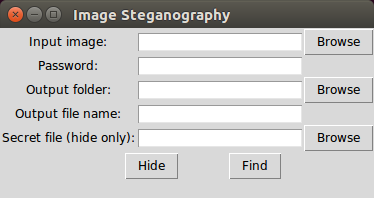
\includegraphics[width=0.6\textwidth]{program_screenshot.png}
        

    \newpage
    \section{Zaključek}

    \newpage
    \printbibliography
     
\end{document}

